\section[势垒贯穿]{势垒贯穿} \label{sec:02.06} % 
% \makebox[5em][s]{} % 短题目拉间距

设质量为$m$的粒子以给定的能量$E=\frac{\hbar^{2}k^{2}}{2m}$自左方入射,遇到图\ref{fig.2-9}所示的势垒:
\begin{equation}\label{eq26.1}
	V(x)=
	\begin{dcases}
		0, 		& x<0,x>a	\\
		V_{0},  & 0\leqslant x \leqslant a
	\end{dcases}
\end{equation}
设$V_{0}>E$,求粒子的运动状态.

\begin{wrapfigure}[9]{r}{8em}
	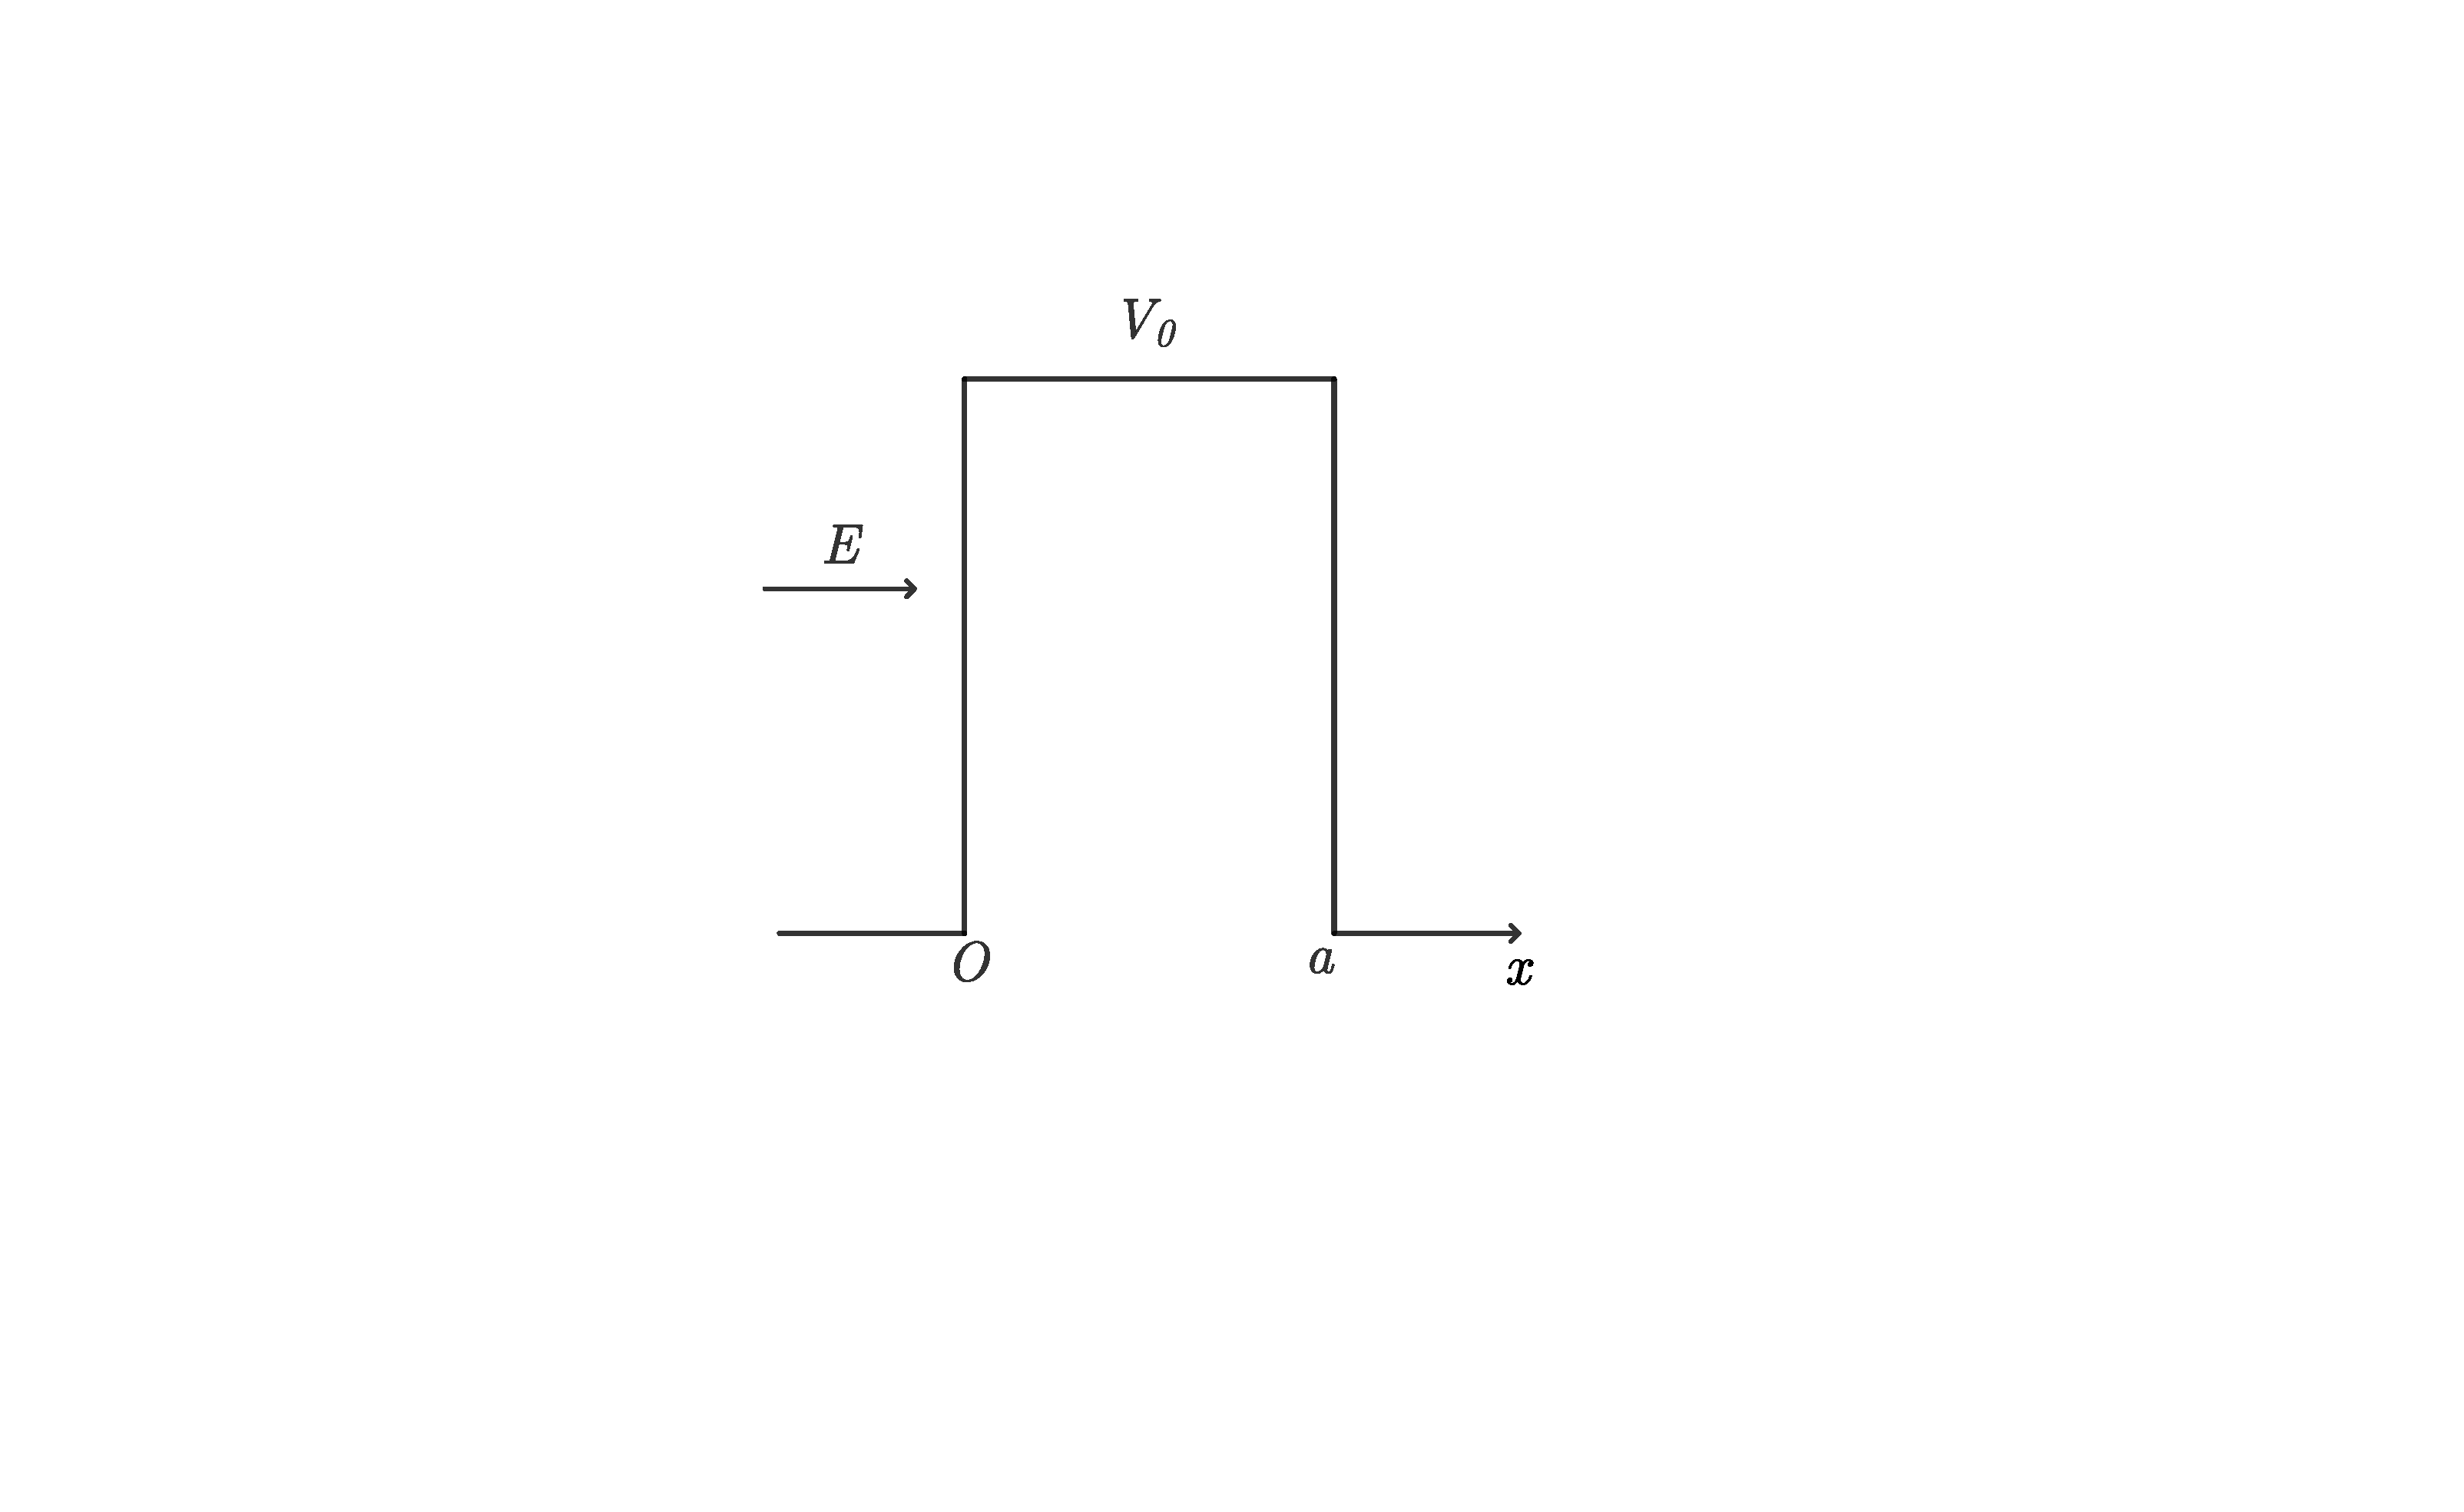
\includegraphics[width=3cm]{QM file/figure/2-9}
	\caption{}\label{fig.2-9}
\end{wrapfigure}

如果是经典力学问题,由于$V_{0}>E$,粒子不能越过势垒,将在$x=0$处被势垒反弹回去.作为量子力学问题,由于粒子的波动性,结论就不一样,可以证明,粒子将有一定概率透过势垒进入$x>a$区域而继续前进.由于粒子的能量是给定的,而且粒子是从$x=-\infty$处射来,这是一个属于游离态的定态问题,波函数可以表示成
\begin{empheq}{equation}\label{eq26.2}
	\varPsi(x,t)=\varPsi(x)e^{-iEt/\hbar}
\end{empheq}
空间波函数$\varPsi(x)$满足定态薛定谔方程:
\begin{empheq}{equation*}\label{eq26.3}
	-\frac{\hbar^{2}}{2m}\varPsi^{\prime\prime}+V(x)\varPsi=E\varPsi=\frac{\hbar^{2}k^{2}}{2m}\varPsi	\tag{2.6.3}
\end{empheq}
亦即
\begin{subnumcases}{}
	\varPsi^{\prime\prime}+k^{2}\varPsi=0,		& x<0,x>a	\label{eq26.3a}\\
	\varPsi^{\prime\prime}-\beta^{2}\varPsi=0,	& 0\leqslant x \leqslant a \label{eq26.3b}
\end{subnumcases}
其中
\begin{empheq}{equation}\label{eq26.4}
	k=\frac{\sqrt{2mE}}{\hbar},\quad \beta=\frac{\sqrt{2m(V_{0}-E)}}{\hbar}
\end{empheq}
\eqref{eq26.3a}式的解为$\varPsi\thicksim e^{\pm ikx}$,考虑到“粒子由左方入射”这个边条件,应取
\begin{subnumcases}{\varPsi(x)=}
	Ae^{ikx}+Re^{-ikx},		& x<0	\label{eq26.5a}\\
	De^{ikx},				& x>a	\label{eq26.5b}
\end{subnumcases}
$A$项为入射波,$R$项为反射波,$D$项为透射波.由于并无粒子从右方入射,所以$x>a$区域没有项$e^{-ikx}$.\eqref{eq26.3b}式的解为
\begin{empheq}{equation*}\label{eq26.5c}
	\varPsi(x)=Be^{\beta x}+Ce^{-\beta x},\quad 0<x<a	\tag{2.6.5c}
\end{empheq}
其中入射波振幅$ A $可以任意给定,其余4个系数可以利用$ x=0 $,a处$\varPsi$和$\varPsi^{\prime\prime}$的连续条件求出.按照\eqref{eq22.9}式及例题,容易求出
\setlength{\mathindent}{6em}
\begin{empheq}{align*}
	\text{入射流量}\quad j_{A}&=|A|^{2}\frac{\hbar k}{m}	\\
	\text{反射流量}\quad j_{R}&=|R|^{2}\bigg( -\frac{\hbar k}{m} \bigg) \\
	\text{透射流量}\quad j_{D}&=|D|^{2}\frac{\hbar k}{m}
\end{empheq}\eqnormal
因此粒子被势垒反射回去的概率(反射系数)和透过势垒的概率(透射系数)为
\begin{equation}\label{eq26.6}
	\begin{aligned}
		\text{反射系数}&=|\frac{j_{R}}{j_{A}}|=|\frac{R}{A}|^{2}	\\
		\text{透射系数}&=|\frac{j_{D}}{j_{A}}|=|\frac{D}{A}|^{2}
	\end{aligned}
\end{equation}
以下求系数$R,D$.$x=0$处$\varPsi(x)$及$\varPsi^{\prime}(x)$应该连续,由\eqref{eq26.5a},\eqref{eq26.5b}式易得
\begin{equation}\label{eq26.7}
	\begin{dcases}
		A+R=B+C	\\
		ik(A-R)=\beta(B-C)
	\end{dcases}
\end{equation}
$x=a$处$\varPsi$及$\varPsi^{\prime}$也应该连续,由\eqref{eq26.5b},\eqref{eq26.5c}式易得
\begin{equation}\label{eq26.8}
	\begin{dcases}
		De^{ika}=Be^{\beta a}+Ce^{-\beta a}	\\
		ikDe^{ika}=\beta Be^{\beta a}-\beta Ce^{-\beta a}
	\end{dcases}
\end{equation}
由\eqref{eq26.7}式可得
\begin{equation}\label{eq26.9}
	\begin{cases}
		\frac{2B}{A}=1+\frac{ik}{\beta}+\bigg(1-\frac{ik}{\beta}\bigg)\frac{R}{A}		\\
		\frac{2C}{A}=1-\frac{ik}{\beta}+\bigg(1+\frac{ik}{\beta}\bigg)\frac{R}{A}	
	\end{cases}
\end{equation}
由(8)式可得
\begin{equation}\label{eq26.10}
	\begin{cases}
		\frac{2B}{A}=\bigg(1+\frac{ik}{\beta}\bigg)\frac{D}{A}e^{-\beta a+ika}		\\
		\frac{2C}{A}=\bigg(1-\frac{ik}{\beta}\bigg)\frac{D}{A}e^{\beta a+ika}	
	\end{cases}
\end{equation}
比较\eqref{eq26.9}、\eqref{eq26.10}式,得到
\begin{equation}\label{eq26.11}
	\begin{cases}
		\gamma+\frac{R}{A}=\frac{D}{A}\gamma e^{-\beta a+ika}		\\
		\gamma^{*}+\frac{R}{A}=\frac{D}{A}\gamma^{*}e^{\beta a+ika}	
	\end{cases}
\end{equation}
其中
\setlength{\mathindent}{5em}
\begin{empheq}{equation}\label{eq26.12}
	\gamma=\frac{\beta+ik}{\beta-ik},\quad \gamma^{*}=\frac{\beta-ik}{\beta+ik}=\frac{1}{\gamma},\quad |\gamma|=1
\end{empheq}
由\eqref{eq26.11}式解出
\begin{empheq}{equation}\label{eq26.13}
	\frac{D}{A}=\frac{(\gamma-\gamma^{*})e^{-ika}}{\gamma e^{-\beta a}-\gamma^{*}e^{\beta a}},\quad
	\frac{R}{A}=\frac{e^{\beta a}-e^{-\beta A}}{\gamma e^{-\beta a}-\gamma^{*}e^{\beta a}}
\end{empheq}
\begin{equation}\label{eq26.14}
	\begin{aligned}
		|\frac{D}{A}|^{2} &=\frac{(\gamma-\gamma^{*})^{2}}{e^{2\beta a}+e^{-2\beta a}-(\gamma^{2}+\gamma^{*2})}	\text{(透射系数)}	\\
		|\frac{R}{A}|^{2} &=\frac{(e^{\beta a}-e^{-\beta a})^{2}}{e^{2\beta a}+e^{-2\beta a}-(\gamma^{2}+\gamma^{*2})}	\text{(反射系数)}
	\end{aligned}
\end{equation}
\eqnormal
利用关系式
\begin{empheq}{equation*}
	|\gamma-\gamma^{*}|^{2}=2-(\gamma^{2}+\gamma^{*2})
\end{empheq}
容易证明
\begin{empheq}{equation}\label{eq26.15}
	|\frac{D}{A}|^{2}+|\frac{R}{A}|^{2}=1
\end{empheq}
这是概率守恒的具体表现形式.

在许多问题中,$e^{2\beta a}\gg 1$,这时\eqref{eq26.14}式分母可以近似取为$e^{2\beta a}$,从而得到
\setlength{\mathindent}{4em}
\begin{empheq}{equation}\label{eq26.16}
	|\frac{D}{A}|^{2}\approx|\gamma-\gamma^{*}|^{2}e^{-2\beta a}
	=\frac{16E(V_{0}-E)}{V_{0}^{2}}e^{-\frac{2a}{\hbar}\sqrt{2m(V_{0}-E)}}
\end{empheq}\eqnormal
这就是$E<V_{0}$时矩形势垒穿透系数的常用公式.为了获得明确的量级概念,举两个简单的例子.

1. 宏观情形,取$m=1\si{g},V_{0}-E=10^{-7}\si{J},a=1\si{cm}$,则
\begin{empheq}{gather*}
	\frac{2a}{\hbar}\sqrt{2m(V_{0}-E)}=\num{2.68}\times10^{27}	\\
	|\frac{D}{A}|^{2}\thicksim e^{-2.68\times10^{27}}\thicksim10^{-1.16\times10^{27}}
\end{empheq}
真是微乎其微!宏观领域从未发现势垒贯穿现象,就是因为概率太小.

2. 微观情形,取$m=m_{e}\text{(电子质量)},V_{0}-E=1\si{eV},a=0.1\si{nm}$,则
\begin{empheq}{gather*}
	\frac{2a}{\hbar}\sqrt{2m(V_{0}-E)}=\num{1.026}	\\
	|\frac{D}{A}|^{2}\thicksim e^{-\frac{2a}{\hbar}\sqrt{2m(V_{0}-E)}}\thicksim e^{-1.026}=\num{0.36}
\end{empheq}
透射概率相当大,由此可见在微观领域势垒贯穿现象是容易发生的.

到\eqref{eq26.15}式为止的结果是严格的,而且不难推广到$E>V_{0}$的情况(包括$V_{0}<0$,即势阱的情况).这种情况下的结果,和光波在折射率不同的几层介质中的传播规律(反射,透射)类似.

当$E>V_{0}$,\eqref{eq26.4}式中$\beta$为虚数,
\begin{empheq}{equation*}\label{eq26.4'}
	\beta=\frac{\sqrt{2m(V_{0}-E)}}{\hbar}=\frac{i\sqrt{E-V_{0}}}{\hbar}=i\alpha	\tag{$2.6.4^{\prime}$}
\end{empheq}
代入\eqref{eq26.12}式
\begin{empheq}{equation*}\label{eq26.12'}
	\gamma=\frac{\alpha+k}{\alpha-k},\quad \gamma^{*}=\frac{\alpha-k}{\alpha+k},\quad 
	\gamma\gamma^{*}=1	\tag{$2.6.12^{\prime}$}
\end{empheq}
\eqref{eq26.13}、\eqref{eq26.14}式中
\setlength{\mathindent}{5em}
\begin{empheq}{equation}\label{eq26.17}
	\begin{aligned}
		e^{\beta a}=e^{-\alpha a},&\quad e^{-\beta a}=e^{-i\alpha a}	\\
		(\gamma-\gamma^{*})^{2}=\bigg(\frac{4\alpha k}{\alpha^{2}-k^{2}}\bigg)^{2},&
		\gamma^{2}+\gamma^{*2}=2+\bigg(\frac{4\alpha k}{\alpha^{2}-k^{2}}\bigg)^{2}
	\end{aligned}
\end{empheq}\eqnormal
在一般情况下,$\alpha,k$量级相同,\eqref{eq26.14}式分子、分母中各项量级也相同,所以反射系数$|\frac{R}{A}|^{2}$与透射系数$|\frac{D}{A}|^{2}$的量级也大致相同,透射很容易.

有一种特殊情况值得注意,如果$e^{i\alpha a}=e^{-i\alpha a}$,即
\begin{empheq}{equation}\label{eq26.18}
	e^{i2\alpha a}=1,\quad \alpha a=\pi,2\pi,3\pi,\cdots
\end{empheq}
由\eqref{eq26.14}式可以看出$R=0$,没有反射,而透射系数$|\frac{D}{A}|^{2}=1$.这种情形称为共振透射.共振条件\eqref{eq26.18}也就是
\setlength{\mathindent}{5em}
\begin{empheq}{equation}\label{eq26.19}
	\frac{2a}{\lambda}=1,2,3,\cdots,\quad \lambda=\frac{2\pi}{\alpha}=\frac{h}{\sqrt{2m(E-V_{0})}}
\end{empheq}\eqnormal
$\lambda$为粒子在势垒(阱)内的物质波波长.

对于一般形状的势垒(见图\ref{fig.2-10}),透射系数的计算较复杂(求解定态薛定谔方程!)但如入射能量$E$较小,$V(x)>E$的区域相当宽,总透射系数很小,则可以用以下的粗略近似处理.

\begin{wrapfigure}[9]{r}{12em}
	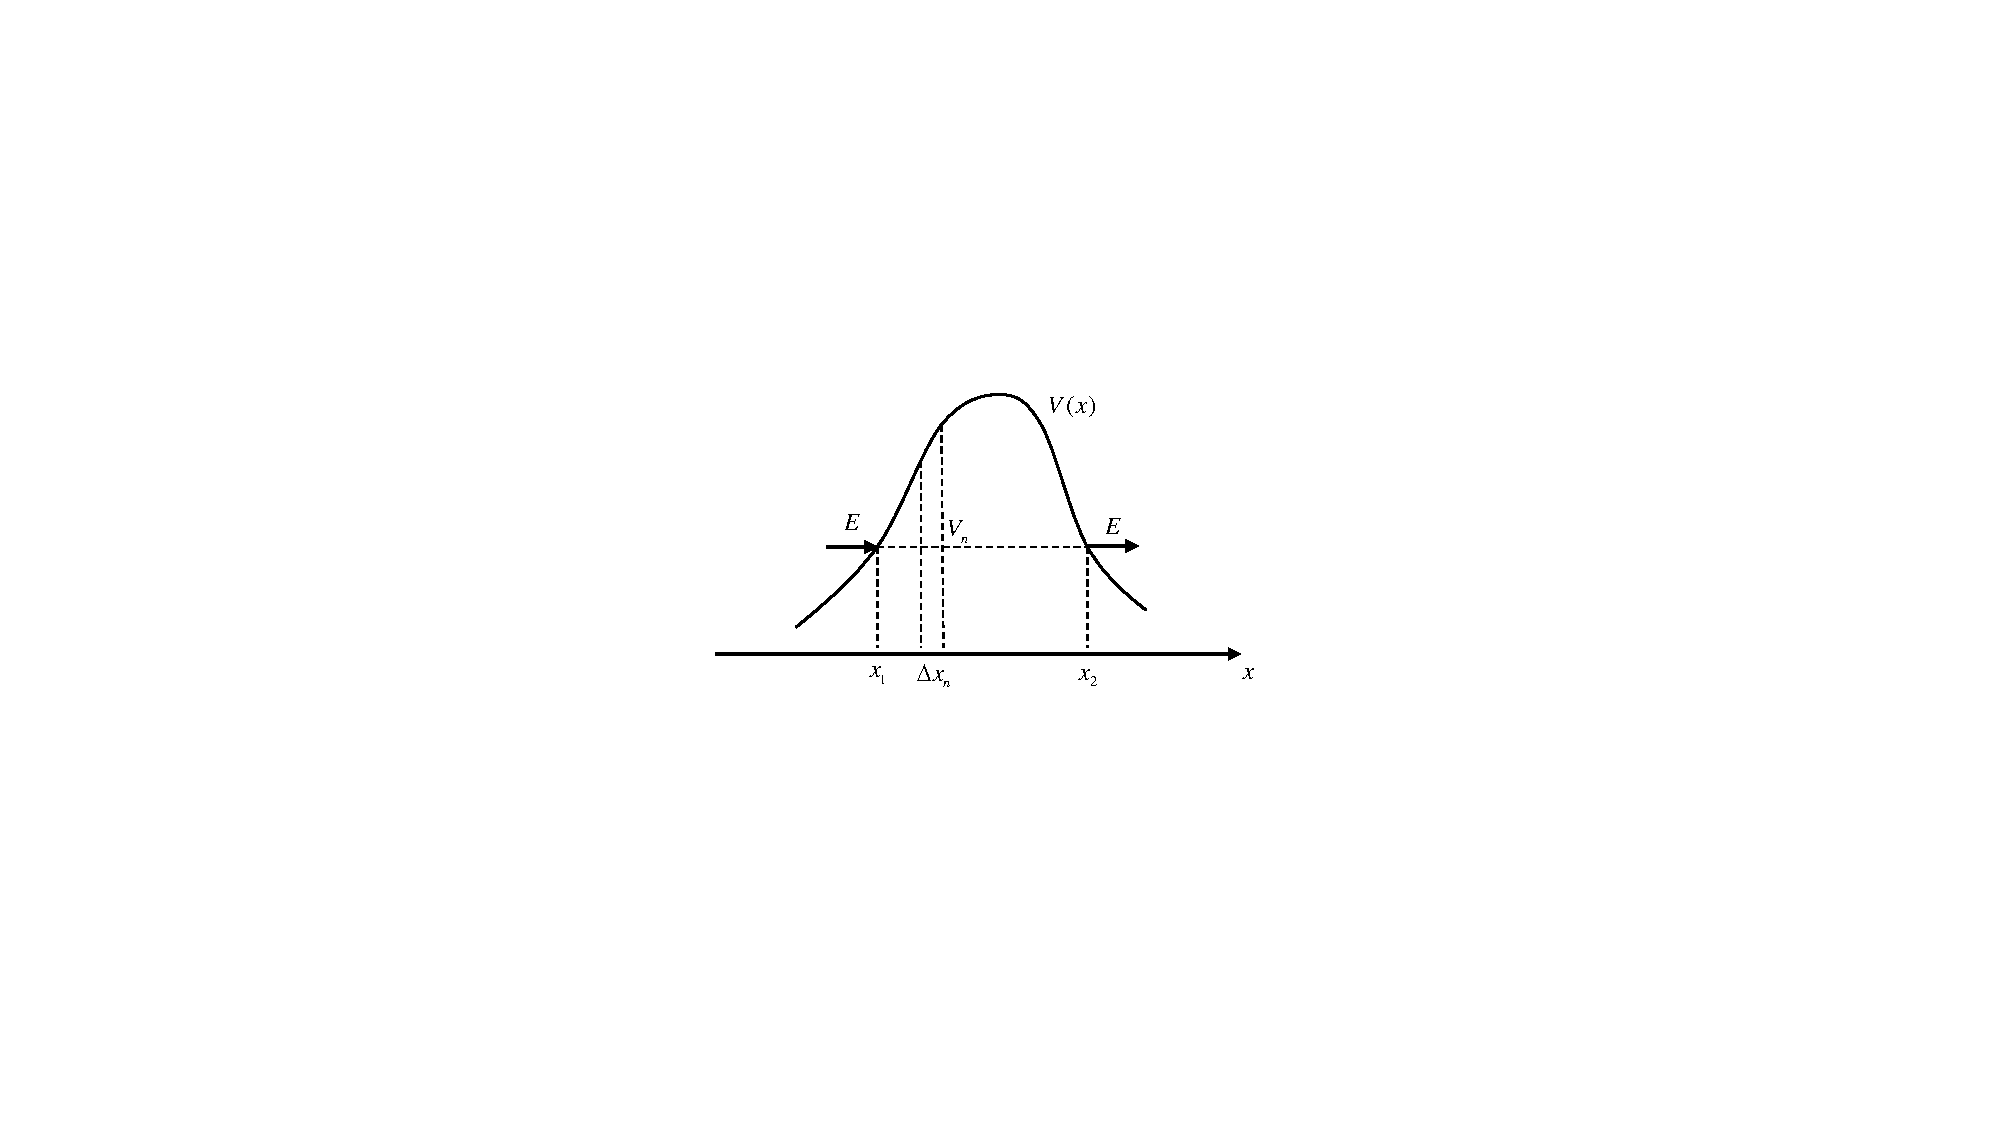
\includegraphics[width=4cm]{QM file/figure/2-10}
	\caption{}\label{fig.2-10}
\end{wrapfigure}

将$V(x)>E$的部分划分成许多窄条(宽$\Delta x_{n}$)状的矩形势垒,粒子对其中一条的穿透概率取为
\setlength{\mathindent}{5em}
\begin{empheq}{equation*}
	e^{\frac{2\Delta x_{n}}{\hbar}\sqrt{2m(V_{0}-E)}}
\end{empheq}\eqnormal
各条穿透概率的乘积等于粒子对整个势垒的总穿透概率.($V<E$的部分,容易穿透,概率按1处理)因此
\setlength{\mathindent}{4em}
\begin{empheq}{equation}\label{eq26.20}
	\text{总穿透概率}\thicksim \exp\big[-\frac{2}{\hbar}\sqrt{2m}\int_{x_{1}}^{x^{2}}\sqrt{V(x)-E}dx\big]
\end{empheq}\eqnormal
$x_{1},x_{2}$为经典回转点,即$V(x_{1})=V(x_{2})=E$.

势垒贯穿现象也称“隧道效应”.诸如原子核的$\alpha$放射性,导体中自由电子的形成,不同导体间的接触电势差, 都与隧道效应有关.20 世纪60年代,利用电子在结型半导体中的隧道效应,制成了有名的隧道二极管.

\example 金属中自由电子的“冷发射”.

在金属表面加一个强电场($\mathscr{E}\thicksim10^{6}\si{V/cm}$)电子就能从金属中逸出,这现象称为冷发射[将金属(阴极)加热而得到电流,称为热发射].这是一种典型的隧道效应.

加外电场前,金属中自由电子所处平均势场大致如图\ref{fig.2-11}(a)所示,$x<0$为金属,$V\approx 0$,$x>0$为真空,$V\approx V_{0}$,$(V_{0}-E)$就是电子逸出金属所需能量(逸出功).由于势垒为半无限宽,电子无法逸出(穿透概率为0).以金属为阴极,加强电场$\mathscr{E}$后,势能变成
\begin{figure}[htbp]
	\centering
	\begin{minipage}{0.49\linewidth}
		\centering
		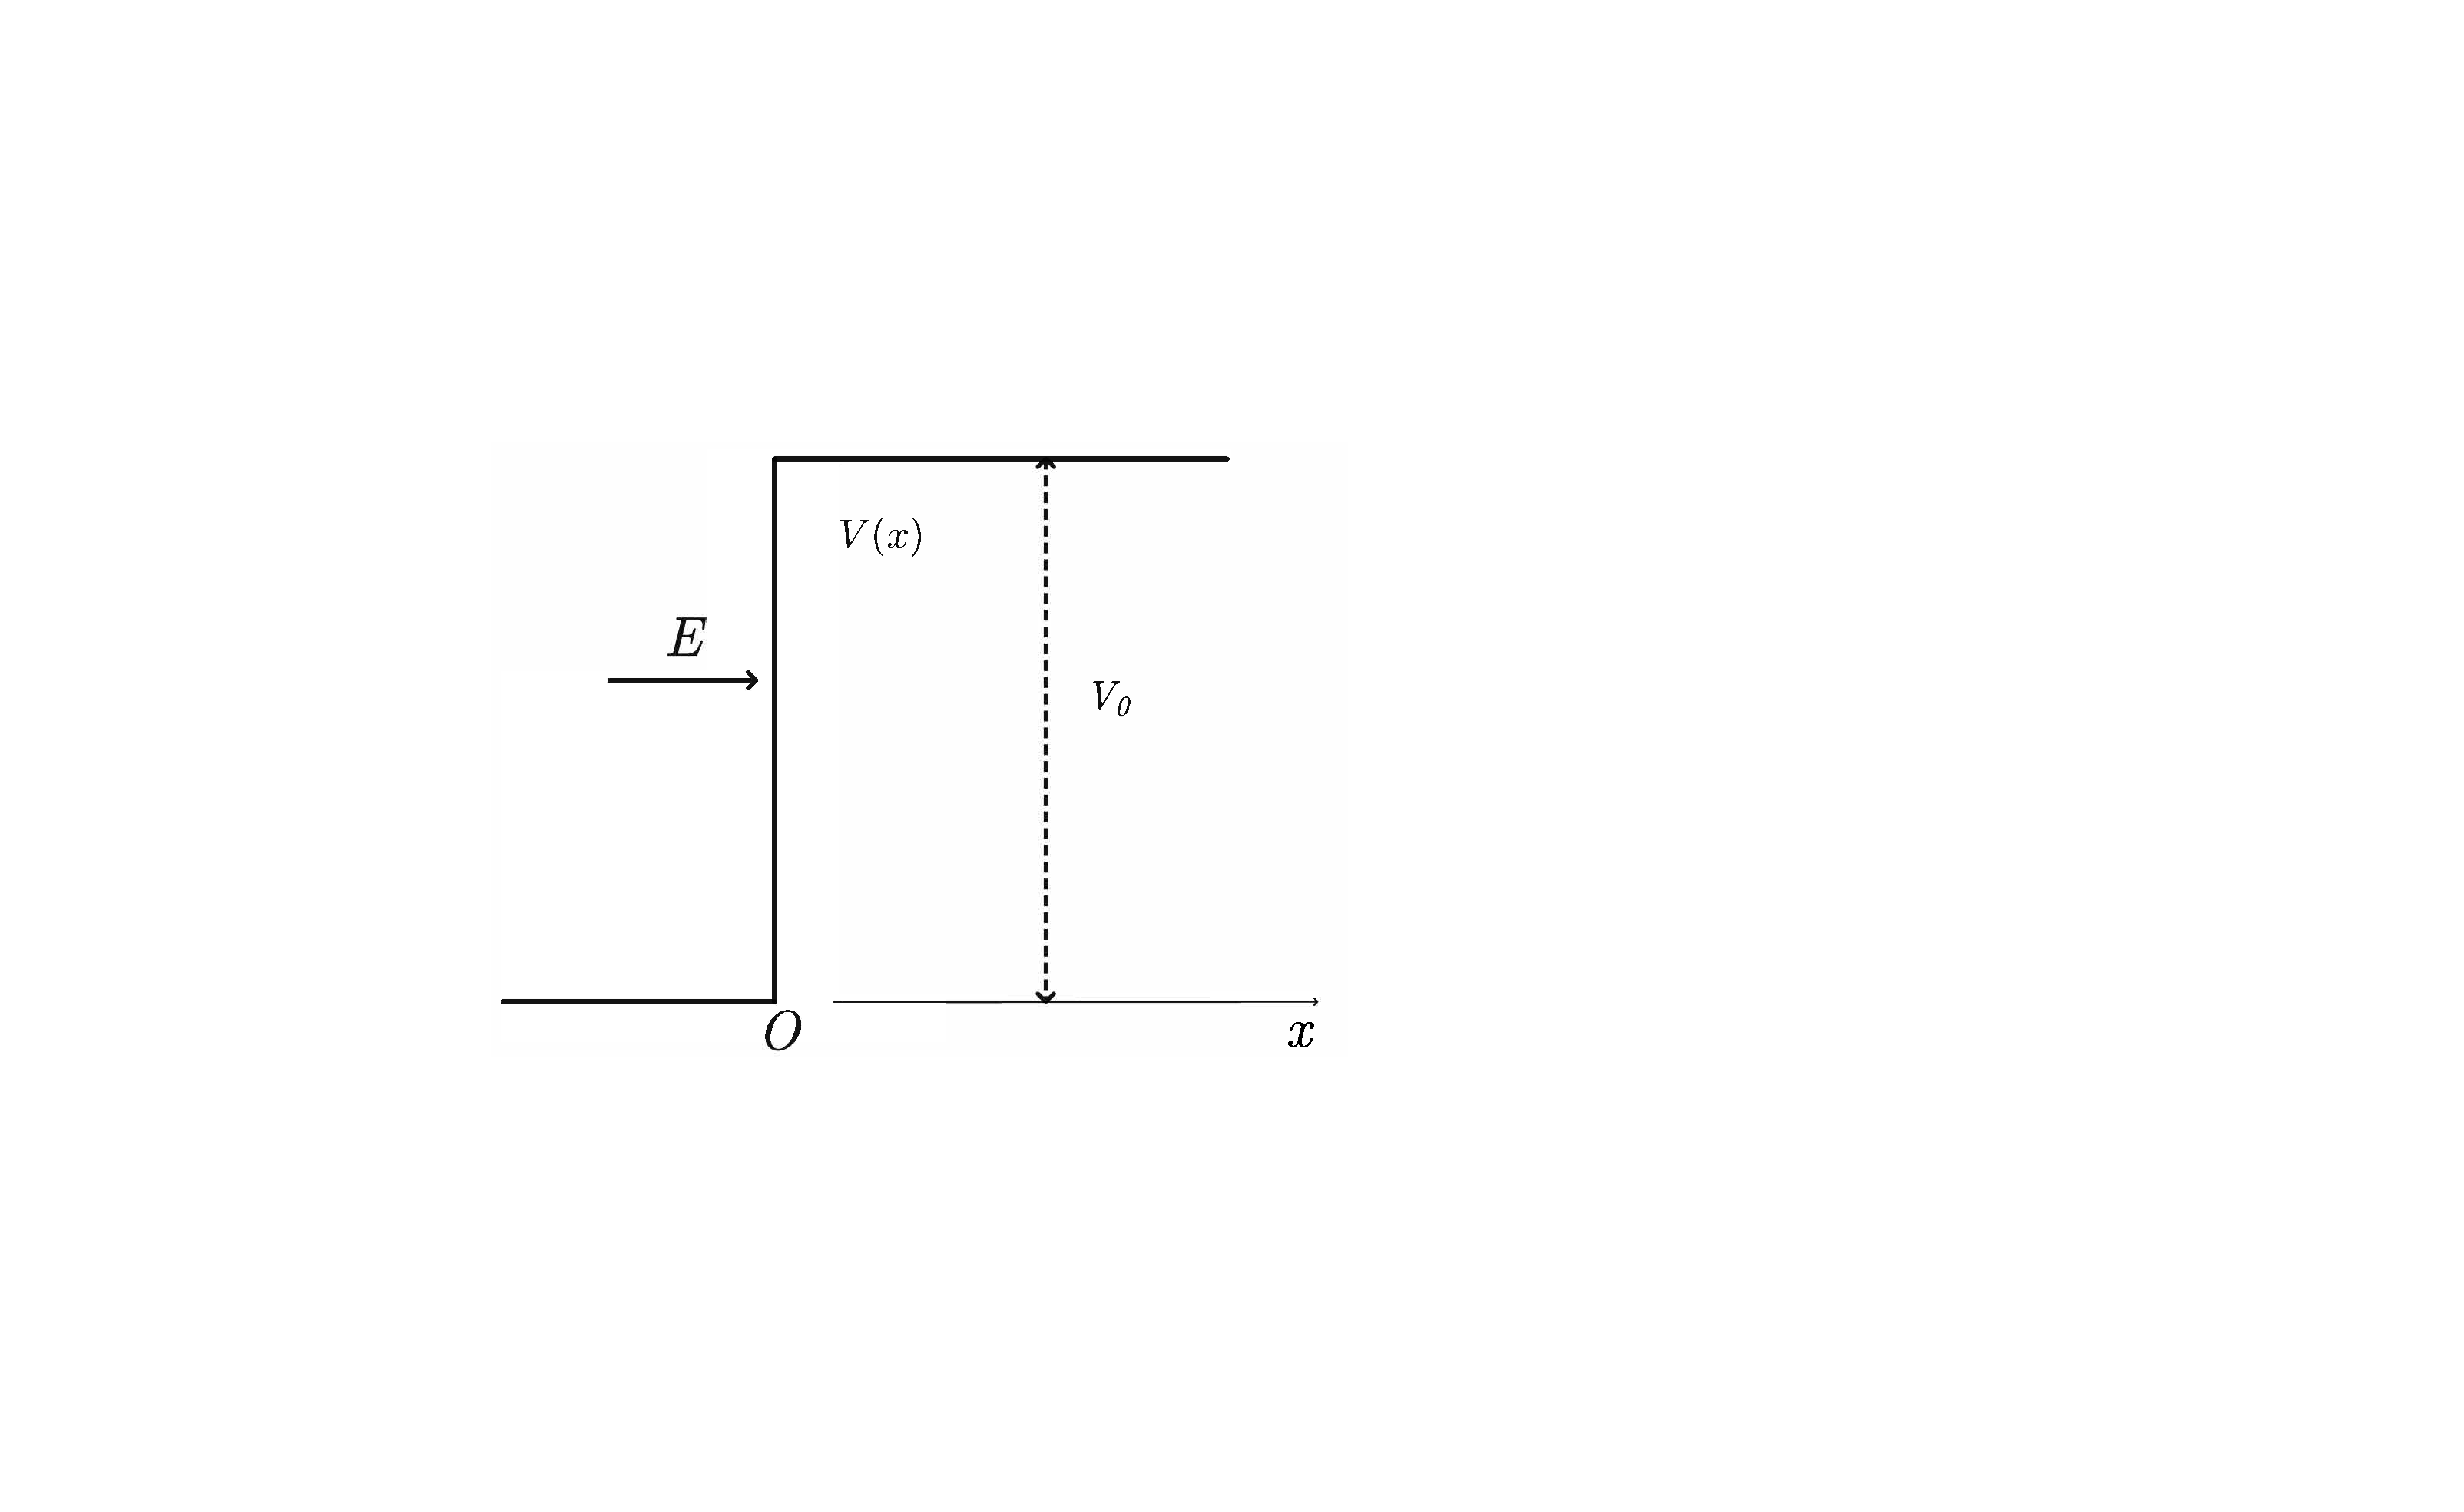
\includegraphics[width=0.6\linewidth]{QM file/figure/2-11(a)}
		\centerline{(a)}
		%\label{fig.2-11(a)}%文中引用该图片代号
	\end{minipage}
	\begin{minipage}{0.49\linewidth}
		\centering
		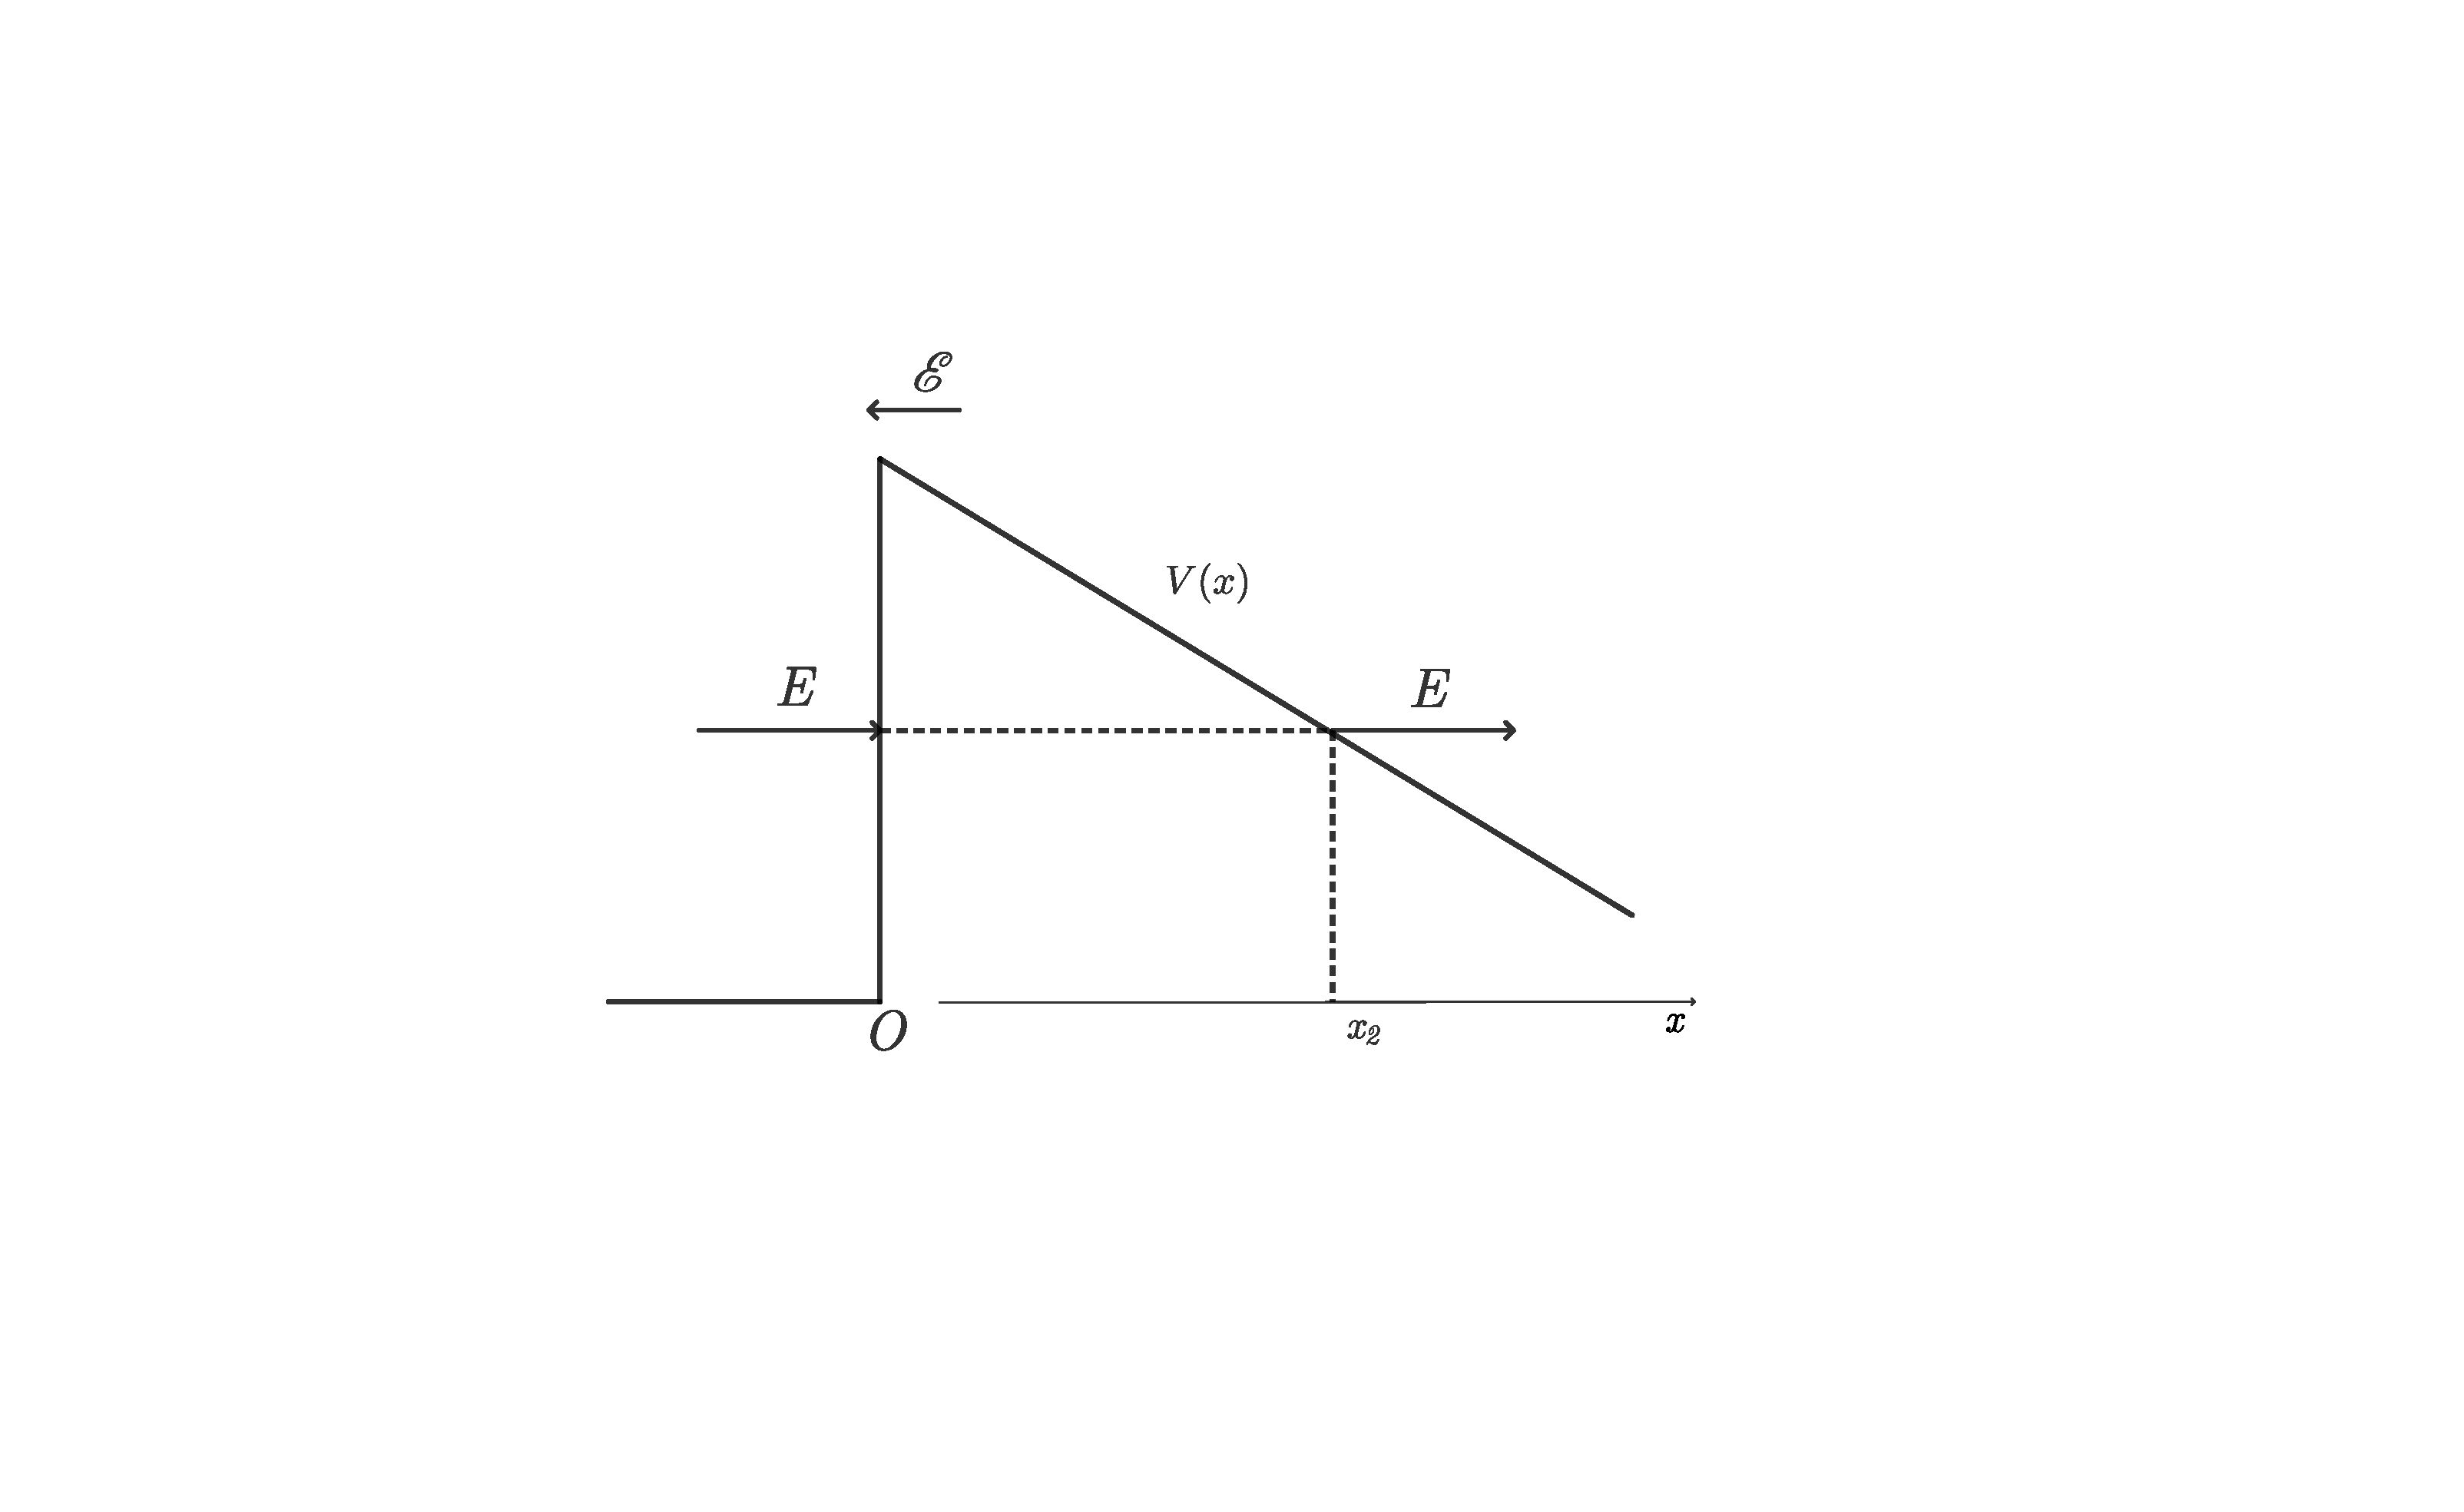
\includegraphics[width=0.6\linewidth]{QM file/figure/2-11(b)}
		\centerline{(b)}
		%\label{fig.2-11(b)}%文中引用该图片代号
	\end{minipage}
	\caption{}\label{fig.2-11}
\end{figure}
\begin{equation}\label{eq26.21}
	V(x)=
	\begin{dcases}
	0,		& x<0	\\	
	V_{0}-e\mathscr{E}x,	& x>0	
	\end{dcases}
\end{equation}
形成图\ref{fig.2-11}(b)所示的三角形势垒按照\eqref{eq26.20}式,电子对势垒的穿透概率约为
\setlength{\mathindent}{5em}
\begin{empheq}{equation}\label{eq26.22}
	exp\big[-\frac{2}{\hbar}\sqrt{2m}\int_{0}^{x^{2}}\sqrt{2m(V_{0}-E-e\mathscr{E}x)}dx\big]
	=e^{-\bar{\mathscr{E}_{0}}/\mathscr{E}}
\end{empheq}
其中
\begin{empheq}{equation}\label{eq26.23}
	x=\frac{(V_{0}-E)}{e\mathscr{E}},\quad \mathscr{E}_{0}=\frac{4}{3e\hbar}=\sqrt{2m}(V_{0}-E)^{\frac{3}{2}}
\end{empheq}\eqnormal
确切说来,金属中自由电子的能量$E$可以在能带范围内取各种不同值,所以\eqref{eq26.22}、\eqref{eq26.23}式还应该作某些统计平均处理.但是\eqref{eq26.22}式已经反映冷发射电流和外电场关系的基本特点,即冷发射电流
\eqshort
\begin{empheq}{equation}\label{eq26.24}
	I=I_{0}e^{-\bar{\mathscr{E}_{0}}/\mathscr{E}}
\end{empheq}\eqnormal
$\bar{\mathscr{E}_{0}}$是$\mathscr{E}_{0}$的某种统计平均值.$I_{0}$和$\bar{\mathscr{E}_{0}}$取决于金属的能带结构性质.\eqref{eq26.24}式和实验结果大致符合.